\documentclass[twoside]{book}

% Packages required by doxygen
\usepackage{fixltx2e}
\usepackage{calc}
\usepackage{doxygen}
\usepackage[export]{adjustbox} % also loads graphicx
\usepackage{graphicx}
\usepackage[utf8]{inputenc}
\usepackage{makeidx}
\usepackage{multicol}
\usepackage{multirow}
\PassOptionsToPackage{warn}{textcomp}
\usepackage{textcomp}
\usepackage[nointegrals]{wasysym}
\usepackage[table]{xcolor}

% Font selection
\usepackage[T1]{fontenc}
\usepackage[scaled=.90]{helvet}
\usepackage{courier}
\usepackage{amssymb}
\usepackage{sectsty}
\renewcommand{\familydefault}{\sfdefault}
\allsectionsfont{%
  \fontseries{bc}\selectfont%
  \color{darkgray}%
}
\renewcommand{\DoxyLabelFont}{%
  \fontseries{bc}\selectfont%
  \color{darkgray}%
}
\newcommand{\+}{\discretionary{\mbox{\scriptsize$\hookleftarrow$}}{}{}}

% Page & text layout
\usepackage{geometry}
\geometry{%
  a4paper,%
  top=2.5cm,%
  bottom=2.5cm,%
  left=2.5cm,%
  right=2.5cm%
}
\tolerance=750
\hfuzz=15pt
\hbadness=750
\setlength{\emergencystretch}{15pt}
\setlength{\parindent}{0cm}
\setlength{\parskip}{3ex plus 2ex minus 2ex}
\makeatletter
\renewcommand{\paragraph}{%
  \@startsection{paragraph}{4}{0ex}{-1.0ex}{1.0ex}{%
    \normalfont\normalsize\bfseries\SS@parafont%
  }%
}
\renewcommand{\subparagraph}{%
  \@startsection{subparagraph}{5}{0ex}{-1.0ex}{1.0ex}{%
    \normalfont\normalsize\bfseries\SS@subparafont%
  }%
}
\makeatother

% Headers & footers
\usepackage{fancyhdr}
\pagestyle{fancyplain}
\fancyhead[LE]{\fancyplain{}{\bfseries\thepage}}
\fancyhead[CE]{\fancyplain{}{}}
\fancyhead[RE]{\fancyplain{}{\bfseries\leftmark}}
\fancyhead[LO]{\fancyplain{}{\bfseries\rightmark}}
\fancyhead[CO]{\fancyplain{}{}}
\fancyhead[RO]{\fancyplain{}{\bfseries\thepage}}
\fancyfoot[LE]{\fancyplain{}{}}
\fancyfoot[CE]{\fancyplain{}{}}
\fancyfoot[RE]{\fancyplain{}{\bfseries\scriptsize Generated by Doxygen }}
\fancyfoot[LO]{\fancyplain{}{\bfseries\scriptsize Generated by Doxygen }}
\fancyfoot[CO]{\fancyplain{}{}}
\fancyfoot[RO]{\fancyplain{}{}}
\renewcommand{\footrulewidth}{0.4pt}
\renewcommand{\chaptermark}[1]{%
  \markboth{#1}{}%
}
\renewcommand{\sectionmark}[1]{%
  \markright{\thesection\ #1}%
}

% Indices & bibliography
\usepackage{natbib}
\usepackage[titles]{tocloft}
\setcounter{tocdepth}{3}
\setcounter{secnumdepth}{5}
\makeindex

% Hyperlinks (required, but should be loaded last)
\usepackage{ifpdf}
\ifpdf
  \usepackage[pdftex,pagebackref=true]{hyperref}
\else
  \usepackage[ps2pdf,pagebackref=true]{hyperref}
\fi
\hypersetup{%
  colorlinks=true,%
  linkcolor=blue,%
  citecolor=blue,%
  unicode%
}

% Custom commands
\newcommand{\clearemptydoublepage}{%
  \newpage{\pagestyle{empty}\cleardoublepage}%
}

\usepackage{caption}
\captionsetup{labelsep=space,justification=centering,font={bf},singlelinecheck=off,skip=4pt,position=top}

%===== C O N T E N T S =====

\begin{document}

% Titlepage & ToC
\hypersetup{pageanchor=false,
             bookmarksnumbered=true,
             pdfencoding=unicode
            }
\pagenumbering{roman}
\begin{titlepage}
\vspace*{7cm}
\begin{center}%
{\Large My Project \\[1ex]\large Midterm project of Rishabh C\+Houdhary and Akash Atharv }\\
\vspace*{1cm}
{\large Generated by Doxygen 1.8.11}\\
\end{center}
\end{titlepage}
\clearemptydoublepage
\tableofcontents
\clearemptydoublepage
\pagenumbering{arabic}
\hypersetup{pageanchor=true}

%--- Begin generated contents ---
\chapter{Hierarchical Index}
\section{Class Hierarchy}
This inheritance list is sorted roughly, but not completely, alphabetically\+:\begin{DoxyCompactList}
\item \contentsline{section}{image\+Processor}{\pageref{classimageProcessor}}{}
\begin{DoxyCompactList}
\item \contentsline{section}{lanes}{\pageref{classlanes}}{}
\end{DoxyCompactList}
\end{DoxyCompactList}

\chapter{Class Index}
\section{Class List}
Here are the classes, structs, unions and interfaces with brief descriptions\+:\begin{DoxyCompactList}
\item\contentsline{section}{\hyperlink{classimageProcessor}{image\+Processor} \\*Class \hyperlink{classimageProcessor}{image\+Processor} The class \hyperlink{classimageProcessor}{image\+Processor} deals with the initial processing algorithms to be performed on the frame before the lines detected are processed further }{\pageref{classimageProcessor}}{}
\item\contentsline{section}{\hyperlink{classlanes}{lanes} \\*Class lanes The class lanes deals with all the operations remaining for lane detection after the hough lines in the image have been detected derived from the base class Image\+Processor }{\pageref{classlanes}}{}
\end{DoxyCompactList}

\chapter{File Index}
\section{File List}
Here is a list of all documented files with brief descriptions\+:\begin{DoxyCompactList}
\item\contentsline{section}{app/\hyperlink{demo_8cpp}{demo.\+cpp} \\*\subsection*{\+: Implements an instance of lane detection application }}{\pageref{demo_8cpp}}{}
\item\contentsline{section}{app/\hyperlink{imageProcessor_8cpp}{image\+Processor.\+cpp} \\*\subsection*{\+: Contains function definitions of the class \hyperlink{classimageProcessor}{image\+Processor} }}{\pageref{imageProcessor_8cpp}}{}
\item\contentsline{section}{app/\hyperlink{lanes_8cpp}{lanes.\+cpp} \\*\subsection*{\+: Contains function definitions of the class lanes }}{\pageref{lanes_8cpp}}{}
\item\contentsline{section}{include/\hyperlink{imageProcessor_8hpp}{image\+Processor.\+hpp} \\*\subsection*{\+: Contains function and variable declarations of the class \hyperlink{classimageProcessor}{image\+Processor} }}{\pageref{imageProcessor_8hpp}}{}
\item\contentsline{section}{include/\hyperlink{lanes_8hpp}{lanes.\+hpp} \\*\subsection*{\+: Contains function and variable definitions of the class lanes }}{\pageref{lanes_8hpp}}{}
\end{DoxyCompactList}

\chapter{Class Documentation}
\hypertarget{classimageProcessor}{}\section{image\+Processor Class Reference}
\label{classimageProcessor}\index{image\+Processor@{image\+Processor}}


Class \hyperlink{classimageProcessor}{image\+Processor} The class \hyperlink{classimageProcessor}{image\+Processor} deals with the initial processing algorithms to be performed on the frame before the lines detected are processed further.  




{\ttfamily \#include $<$image\+Processor.\+hpp$>$}



Inheritance diagram for image\+Processor\+:
\nopagebreak
\begin{figure}[H]
\begin{center}
\leavevmode
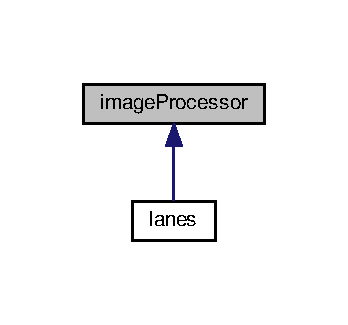
\includegraphics[width=167pt]{classimageProcessor__inherit__graph}
\end{center}
\end{figure}
\subsection*{Public Member Functions}
\begin{DoxyCompactItemize}
\item 
\hyperlink{classimageProcessor_ab81b2da5eb762b48e52824e29dd6b263}{image\+Processor} ()
\begin{DoxyCompactList}\small\item\em constructor for \hyperlink{classimageProcessor}{image\+Processor} \end{DoxyCompactList}\item 
virtual \hyperlink{classimageProcessor_a569b7fd659354a79035dd808f407e34f}{$\sim$image\+Processor} ()
\begin{DoxyCompactList}\small\item\em destructor for \hyperlink{classimageProcessor}{image\+Processor} \end{DoxyCompactList}\item 
cv\+::\+Mat \hyperlink{classimageProcessor_ae353d4dda0b4cac02d8d24d13ea564cd}{get\+Original\+Image} ()
\begin{DoxyCompactList}\small\item\em function for retrieving original frame \end{DoxyCompactList}\item 
cv\+::\+Mat \hyperlink{classimageProcessor_a760757a7f70dc75844a23de9aaa56ea2}{get\+Gray\+Image} ()
\begin{DoxyCompactList}\small\item\em function for retrieving grayscale frame \end{DoxyCompactList}\item 
cv\+::\+Mat \hyperlink{classimageProcessor_a89562102bef26b8b558d43f71cb5dba1}{get\+Noise\+Image} ()
\begin{DoxyCompactList}\small\item\em function for retrieving Noise filtered frame \end{DoxyCompactList}\item 
cv\+::\+Mat \hyperlink{classimageProcessor_aa8a061deb1036ab029445ff5f9e96c06}{get\+Egde\+Image} ()
\begin{DoxyCompactList}\small\item\em function for retrieving edge detected frame \end{DoxyCompactList}\item 
cv\+::\+Mat \hyperlink{classimageProcessor_a4265122d10d5db7962f27f97a1c60d63}{get\+Hough\+Image} ()
\begin{DoxyCompactList}\small\item\em function for retrieving Hough transformed frame \end{DoxyCompactList}\item 
void \hyperlink{classimageProcessor_a95a83955f7a69f5e4d1b74030e32a27f}{set\+Original\+Image} (cv\+::\+Mat)
\begin{DoxyCompactList}\small\item\em function for retrieving and setting the captured frame from video as input image \end{DoxyCompactList}\item 
cv\+::\+Mat \hyperlink{classimageProcessor_abfe9be72666f5779b2abe3df018442cf}{rgb\+To\+Gray} (cv\+::\+Mat)
\begin{DoxyCompactList}\small\item\em converts rgb image to grayscale image \end{DoxyCompactList}\item 
cv\+::\+Mat \hyperlink{classimageProcessor_a704c39f5acb8f8f05f711300de0b4d81}{gray\+To\+R\+GB} (cv\+::\+Mat)
\begin{DoxyCompactList}\small\item\em converts grayscale image to rgb image \end{DoxyCompactList}\item 
cv\+::\+Mat \hyperlink{classimageProcessor_ad2578845d7ece8d5e187eddad9fa2b09}{noise\+Filter} (cv\+::\+Mat)
\begin{DoxyCompactList}\small\item\em filters noise from given input image \end{DoxyCompactList}\item 
cv\+::\+Mat \hyperlink{classimageProcessor_a2be1acf803ab26d3ba83a668f9a7a987}{edge\+Detector} (cv\+::\+Mat)
\begin{DoxyCompactList}\small\item\em detect edges from input image \end{DoxyCompactList}\item 
std\+::vector$<$ cv\+::\+Vec4i $>$ \hyperlink{classimageProcessor_a8718011326c36251f8e1607694d21523}{hough\+Transform} (cv\+::\+Mat, cv\+::\+Mat)
\begin{DoxyCompactList}\small\item\em generate lines from roi image \end{DoxyCompactList}\end{DoxyCompactItemize}


\subsection{Detailed Description}
Class \hyperlink{classimageProcessor}{image\+Processor} The class \hyperlink{classimageProcessor}{image\+Processor} deals with the initial processing algorithms to be performed on the frame before the lines detected are processed further. 

\subsection{Constructor \& Destructor Documentation}
\index{image\+Processor@{image\+Processor}!image\+Processor@{image\+Processor}}
\index{image\+Processor@{image\+Processor}!image\+Processor@{image\+Processor}}
\subsubsection[{\texorpdfstring{image\+Processor()}{imageProcessor()}}]{\setlength{\rightskip}{0pt plus 5cm}image\+Processor\+::image\+Processor (
\begin{DoxyParamCaption}
{}
\end{DoxyParamCaption}
)}\hypertarget{classimageProcessor_ab81b2da5eb762b48e52824e29dd6b263}{}\label{classimageProcessor_ab81b2da5eb762b48e52824e29dd6b263}


constructor for \hyperlink{classimageProcessor}{image\+Processor} 


\begin{DoxyParams}{Parameters}
{\em none} & \\
\hline
\end{DoxyParams}
\begin{DoxyReturn}{Returns}
none 
\end{DoxyReturn}
\index{image\+Processor@{image\+Processor}!````~image\+Processor@{$\sim$image\+Processor}}
\index{````~image\+Processor@{$\sim$image\+Processor}!image\+Processor@{image\+Processor}}
\subsubsection[{\texorpdfstring{$\sim$image\+Processor()}{~imageProcessor()}}]{\setlength{\rightskip}{0pt plus 5cm}image\+Processor\+::$\sim$image\+Processor (
\begin{DoxyParamCaption}
{}
\end{DoxyParamCaption}
)\hspace{0.3cm}{\ttfamily [virtual]}}\hypertarget{classimageProcessor_a569b7fd659354a79035dd808f407e34f}{}\label{classimageProcessor_a569b7fd659354a79035dd808f407e34f}


destructor for \hyperlink{classimageProcessor}{image\+Processor} 


\begin{DoxyParams}{Parameters}
{\em none} & \\
\hline
\end{DoxyParams}
\begin{DoxyReturn}{Returns}
none 
\end{DoxyReturn}


\subsection{Member Function Documentation}
\index{image\+Processor@{image\+Processor}!edge\+Detector@{edge\+Detector}}
\index{edge\+Detector@{edge\+Detector}!image\+Processor@{image\+Processor}}
\subsubsection[{\texorpdfstring{edge\+Detector(cv\+::\+Mat)}{edgeDetector(cv::Mat)}}]{\setlength{\rightskip}{0pt plus 5cm}cv\+::\+Mat image\+Processor\+::edge\+Detector (
\begin{DoxyParamCaption}
\item[{cv\+::\+Mat}]{noise\+Image}
\end{DoxyParamCaption}
)}\hypertarget{classimageProcessor_a2be1acf803ab26d3ba83a668f9a7a987}{}\label{classimageProcessor_a2be1acf803ab26d3ba83a668f9a7a987}


detect edges from input image 


\begin{DoxyParams}{Parameters}
{\em input} & noise filtered image \\
\hline
\end{DoxyParams}
\begin{DoxyReturn}{Returns}
output edge detected image 
\end{DoxyReturn}
\index{image\+Processor@{image\+Processor}!get\+Egde\+Image@{get\+Egde\+Image}}
\index{get\+Egde\+Image@{get\+Egde\+Image}!image\+Processor@{image\+Processor}}
\subsubsection[{\texorpdfstring{get\+Egde\+Image()}{getEgdeImage()}}]{\setlength{\rightskip}{0pt plus 5cm}cv\+::\+Mat image\+Processor\+::get\+Egde\+Image (
\begin{DoxyParamCaption}
{}
\end{DoxyParamCaption}
)}\hypertarget{classimageProcessor_aa8a061deb1036ab029445ff5f9e96c06}{}\label{classimageProcessor_aa8a061deb1036ab029445ff5f9e96c06}


function for retrieving edge detected frame 


\begin{DoxyParams}{Parameters}
{\em none} & \\
\hline
\end{DoxyParams}
\begin{DoxyReturn}{Returns}
Image after edge detection 
\end{DoxyReturn}
\index{image\+Processor@{image\+Processor}!get\+Gray\+Image@{get\+Gray\+Image}}
\index{get\+Gray\+Image@{get\+Gray\+Image}!image\+Processor@{image\+Processor}}
\subsubsection[{\texorpdfstring{get\+Gray\+Image()}{getGrayImage()}}]{\setlength{\rightskip}{0pt plus 5cm}cv\+::\+Mat image\+Processor\+::get\+Gray\+Image (
\begin{DoxyParamCaption}
{}
\end{DoxyParamCaption}
)}\hypertarget{classimageProcessor_a760757a7f70dc75844a23de9aaa56ea2}{}\label{classimageProcessor_a760757a7f70dc75844a23de9aaa56ea2}


function for retrieving grayscale frame 


\begin{DoxyParams}{Parameters}
{\em none} & \\
\hline
\end{DoxyParams}
\begin{DoxyReturn}{Returns}
Grayscale image 
\end{DoxyReturn}
\index{image\+Processor@{image\+Processor}!get\+Hough\+Image@{get\+Hough\+Image}}
\index{get\+Hough\+Image@{get\+Hough\+Image}!image\+Processor@{image\+Processor}}
\subsubsection[{\texorpdfstring{get\+Hough\+Image()}{getHoughImage()}}]{\setlength{\rightskip}{0pt plus 5cm}cv\+::\+Mat image\+Processor\+::get\+Hough\+Image (
\begin{DoxyParamCaption}
{}
\end{DoxyParamCaption}
)}\hypertarget{classimageProcessor_a4265122d10d5db7962f27f97a1c60d63}{}\label{classimageProcessor_a4265122d10d5db7962f27f97a1c60d63}


function for retrieving Hough transformed frame 


\begin{DoxyParams}{Parameters}
{\em none} & \\
\hline
\end{DoxyParams}
\begin{DoxyReturn}{Returns}
Image with Hough transform generated lines 
\end{DoxyReturn}
\index{image\+Processor@{image\+Processor}!get\+Noise\+Image@{get\+Noise\+Image}}
\index{get\+Noise\+Image@{get\+Noise\+Image}!image\+Processor@{image\+Processor}}
\subsubsection[{\texorpdfstring{get\+Noise\+Image()}{getNoiseImage()}}]{\setlength{\rightskip}{0pt plus 5cm}cv\+::\+Mat image\+Processor\+::get\+Noise\+Image (
\begin{DoxyParamCaption}
{}
\end{DoxyParamCaption}
)}\hypertarget{classimageProcessor_a89562102bef26b8b558d43f71cb5dba1}{}\label{classimageProcessor_a89562102bef26b8b558d43f71cb5dba1}


function for retrieving Noise filtered frame 


\begin{DoxyParams}{Parameters}
{\em none} & \\
\hline
\end{DoxyParams}
\begin{DoxyReturn}{Returns}
Noise filtered image 
\end{DoxyReturn}
\index{image\+Processor@{image\+Processor}!get\+Original\+Image@{get\+Original\+Image}}
\index{get\+Original\+Image@{get\+Original\+Image}!image\+Processor@{image\+Processor}}
\subsubsection[{\texorpdfstring{get\+Original\+Image()}{getOriginalImage()}}]{\setlength{\rightskip}{0pt plus 5cm}cv\+::\+Mat image\+Processor\+::get\+Original\+Image (
\begin{DoxyParamCaption}
{}
\end{DoxyParamCaption}
)}\hypertarget{classimageProcessor_ae353d4dda0b4cac02d8d24d13ea564cd}{}\label{classimageProcessor_ae353d4dda0b4cac02d8d24d13ea564cd}


function for retrieving original frame 


\begin{DoxyParams}{Parameters}
{\em none} & \\
\hline
\end{DoxyParams}
\begin{DoxyReturn}{Returns}
original input image 
\end{DoxyReturn}
\index{image\+Processor@{image\+Processor}!gray\+To\+R\+GB@{gray\+To\+R\+GB}}
\index{gray\+To\+R\+GB@{gray\+To\+R\+GB}!image\+Processor@{image\+Processor}}
\subsubsection[{\texorpdfstring{gray\+To\+R\+G\+B(cv\+::\+Mat)}{grayToRGB(cv::Mat)}}]{\setlength{\rightskip}{0pt plus 5cm}cv\+::\+Mat image\+Processor\+::gray\+To\+R\+GB (
\begin{DoxyParamCaption}
\item[{cv\+::\+Mat}]{edge\+Image}
\end{DoxyParamCaption}
)}\hypertarget{classimageProcessor_a704c39f5acb8f8f05f711300de0b4d81}{}\label{classimageProcessor_a704c39f5acb8f8f05f711300de0b4d81}


converts grayscale image to rgb image 


\begin{DoxyParams}{Parameters}
{\em input} & grayscale image \\
\hline
\end{DoxyParams}
\begin{DoxyReturn}{Returns}
output rgb image 
\end{DoxyReturn}
\index{image\+Processor@{image\+Processor}!hough\+Transform@{hough\+Transform}}
\index{hough\+Transform@{hough\+Transform}!image\+Processor@{image\+Processor}}
\subsubsection[{\texorpdfstring{hough\+Transform(cv\+::\+Mat, cv\+::\+Mat)}{houghTransform(cv::Mat, cv::Mat)}}]{\setlength{\rightskip}{0pt plus 5cm}std\+::vector$<$ cv\+::\+Vec4i $>$ image\+Processor\+::hough\+Transform (
\begin{DoxyParamCaption}
\item[{cv\+::\+Mat}]{mask\+Image, }
\item[{cv\+::\+Mat}]{hough\+Image}
\end{DoxyParamCaption}
)}\hypertarget{classimageProcessor_a8718011326c36251f8e1607694d21523}{}\label{classimageProcessor_a8718011326c36251f8e1607694d21523}


generate lines from roi image 


\begin{DoxyParams}{Parameters}
{\em roi} & image \\
\hline
\end{DoxyParams}
\begin{DoxyReturn}{Returns}
output lines 
\end{DoxyReturn}
\index{image\+Processor@{image\+Processor}!noise\+Filter@{noise\+Filter}}
\index{noise\+Filter@{noise\+Filter}!image\+Processor@{image\+Processor}}
\subsubsection[{\texorpdfstring{noise\+Filter(cv\+::\+Mat)}{noiseFilter(cv::Mat)}}]{\setlength{\rightskip}{0pt plus 5cm}cv\+::\+Mat image\+Processor\+::noise\+Filter (
\begin{DoxyParamCaption}
\item[{cv\+::\+Mat}]{gray\+Image}
\end{DoxyParamCaption}
)}\hypertarget{classimageProcessor_ad2578845d7ece8d5e187eddad9fa2b09}{}\label{classimageProcessor_ad2578845d7ece8d5e187eddad9fa2b09}


filters noise from given input image 


\begin{DoxyParams}{Parameters}
{\em input} & grayscale image \\
\hline
\end{DoxyParams}
\begin{DoxyReturn}{Returns}
noise filtered image 
\end{DoxyReturn}
\index{image\+Processor@{image\+Processor}!rgb\+To\+Gray@{rgb\+To\+Gray}}
\index{rgb\+To\+Gray@{rgb\+To\+Gray}!image\+Processor@{image\+Processor}}
\subsubsection[{\texorpdfstring{rgb\+To\+Gray(cv\+::\+Mat)}{rgbToGray(cv::Mat)}}]{\setlength{\rightskip}{0pt plus 5cm}cv\+::\+Mat image\+Processor\+::rgb\+To\+Gray (
\begin{DoxyParamCaption}
\item[{cv\+::\+Mat}]{original\+Image}
\end{DoxyParamCaption}
)}\hypertarget{classimageProcessor_abfe9be72666f5779b2abe3df018442cf}{}\label{classimageProcessor_abfe9be72666f5779b2abe3df018442cf}


converts rgb image to grayscale image 


\begin{DoxyParams}{Parameters}
{\em input} & rgb image \\
\hline
\end{DoxyParams}
\begin{DoxyReturn}{Returns}
output grayscale image 
\end{DoxyReturn}
\index{image\+Processor@{image\+Processor}!set\+Original\+Image@{set\+Original\+Image}}
\index{set\+Original\+Image@{set\+Original\+Image}!image\+Processor@{image\+Processor}}
\subsubsection[{\texorpdfstring{set\+Original\+Image(cv\+::\+Mat)}{setOriginalImage(cv::Mat)}}]{\setlength{\rightskip}{0pt plus 5cm}void image\+Processor\+::set\+Original\+Image (
\begin{DoxyParamCaption}
\item[{cv\+::\+Mat}]{image}
\end{DoxyParamCaption}
)}\hypertarget{classimageProcessor_a95a83955f7a69f5e4d1b74030e32a27f}{}\label{classimageProcessor_a95a83955f7a69f5e4d1b74030e32a27f}


function for retrieving and setting the captured frame from video as input image 


\begin{DoxyParams}{Parameters}
{\em original} & input frame \\
\hline
\end{DoxyParams}
\begin{DoxyReturn}{Returns}
none 
\end{DoxyReturn}


The documentation for this class was generated from the following files\+:\begin{DoxyCompactItemize}
\item 
include/\hyperlink{imageProcessor_8hpp}{image\+Processor.\+hpp}\item 
app/\hyperlink{imageProcessor_8cpp}{image\+Processor.\+cpp}\end{DoxyCompactItemize}

\hypertarget{classlanes}{}\section{lanes Class Reference}
\label{classlanes}\index{lanes@{lanes}}


Class lanes The class lanes deals with all the operations remaining for lane detection after the hough lines in the image have been detected derived from the base class Image\+Processor.  




{\ttfamily \#include $<$lanes.\+hpp$>$}



Inheritance diagram for lanes\+:
\nopagebreak
\begin{figure}[H]
\begin{center}
\leavevmode
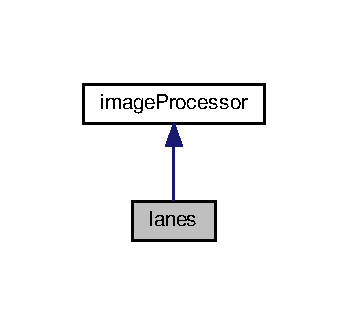
\includegraphics[width=167pt]{classlanes__inherit__graph}
\end{center}
\end{figure}


Collaboration diagram for lanes\+:
\nopagebreak
\begin{figure}[H]
\begin{center}
\leavevmode
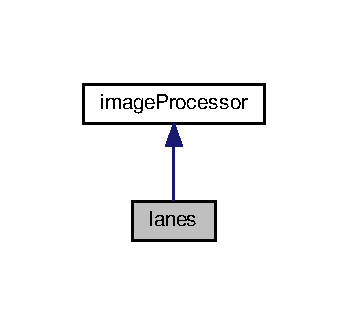
\includegraphics[width=167pt]{classlanes__coll__graph}
\end{center}
\end{figure}
\subsection*{Public Member Functions}
\begin{DoxyCompactItemize}
\item 
\hyperlink{classlanes_a81d66bf4687275c3c09d048f662b7bf4}{lanes} ()
\begin{DoxyCompactList}\small\item\em constructor for lanes \end{DoxyCompactList}\item 
\hyperlink{classlanes_a00021e14af3a9b14ff5f4b92baa18ab4}{$\sim$lanes} ()
\begin{DoxyCompactList}\small\item\em destructor for lanes \end{DoxyCompactList}\item 
std\+::vector$<$ cv\+::\+Vec4i $>$ \hyperlink{classlanes_a7ecd628c303d1e2a25db6edce7f6f3a9}{get\+Left\+Lines} ()
\begin{DoxyCompactList}\small\item\em function for retrieving set of lines detected on left side \end{DoxyCompactList}\item 
std\+::vector$<$ cv\+::\+Vec4i $>$ \hyperlink{classlanes_a8a1607edfaf2ecd2bbf308c59161200a}{get\+Right\+Lines} ()
\begin{DoxyCompactList}\small\item\em function for retrieving set of lines detected on right side \end{DoxyCompactList}\item 
cv\+::\+Mat \hyperlink{classlanes_a69b92f837457006aa91ea332ce9c24c4}{line\+Separation} (std\+::vector$<$ cv\+::\+Vec4i $>$, cv\+::\+Mat)
\begin{DoxyCompactList}\small\item\em function to separate left and right lines on the road \end{DoxyCompactList}\item 
std\+::vector$<$ cv\+::\+Point $>$ \hyperlink{classlanes_a91271ec5b3d5fcc173d640969495d3a6}{fit\+Line} (std\+::vector$<$ cv\+::\+Point $>$, std\+::vector$<$ cv\+::\+Point $>$)
\begin{DoxyCompactList}\small\item\em function to calculate linear regression of given points on left and right lines. \end{DoxyCompactList}\item 
std\+::string \hyperlink{classlanes_afa50aa97e8d8a898553bfd05e2ccb791}{lane\+Prediction} (cv\+::\+Vec4f, cv\+::\+Vec4f, std\+::vector$<$ cv\+::\+Point $>$)
\begin{DoxyCompactList}\small\item\em function to predict lane heading given left anf right line \end{DoxyCompactList}\item 
void \hyperlink{classlanes_ab46f8c8cd6a5109d5cafe1cb591a4edf}{show\+Output} (std\+::string, cv\+::\+Mat, std\+::vector$<$ cv\+::\+Point $>$)
\begin{DoxyCompactList}\small\item\em function for displaying the output \end{DoxyCompactList}\end{DoxyCompactItemize}
\subsection*{Public Attributes}
\begin{DoxyCompactItemize}
\item 
std\+::string {\bfseries prediction}\hypertarget{classlanes_af44823fc2f1e0fe31c26ec6c4c409f26}{}\label{classlanes_af44823fc2f1e0fe31c26ec6c4c409f26}

\end{DoxyCompactItemize}


\subsection{Detailed Description}
Class lanes The class lanes deals with all the operations remaining for lane detection after the hough lines in the image have been detected derived from the base class Image\+Processor. 

\subsection{Constructor \& Destructor Documentation}
\index{lanes@{lanes}!lanes@{lanes}}
\index{lanes@{lanes}!lanes@{lanes}}
\subsubsection[{\texorpdfstring{lanes()}{lanes()}}]{\setlength{\rightskip}{0pt plus 5cm}lanes\+::lanes (
\begin{DoxyParamCaption}
{}
\end{DoxyParamCaption}
)}\hypertarget{classlanes_a81d66bf4687275c3c09d048f662b7bf4}{}\label{classlanes_a81d66bf4687275c3c09d048f662b7bf4}


constructor for lanes 


\begin{DoxyParams}{Parameters}
{\em none} & \\
\hline
\end{DoxyParams}
\begin{DoxyReturn}{Returns}
none 
\end{DoxyReturn}
\index{lanes@{lanes}!````~lanes@{$\sim$lanes}}
\index{````~lanes@{$\sim$lanes}!lanes@{lanes}}
\subsubsection[{\texorpdfstring{$\sim$lanes()}{~lanes()}}]{\setlength{\rightskip}{0pt plus 5cm}lanes\+::$\sim$lanes (
\begin{DoxyParamCaption}
{}
\end{DoxyParamCaption}
)}\hypertarget{classlanes_a00021e14af3a9b14ff5f4b92baa18ab4}{}\label{classlanes_a00021e14af3a9b14ff5f4b92baa18ab4}


destructor for lanes 


\begin{DoxyParams}{Parameters}
{\em none} & \\
\hline
\end{DoxyParams}
\begin{DoxyReturn}{Returns}
none 
\end{DoxyReturn}


\subsection{Member Function Documentation}
\index{lanes@{lanes}!fit\+Line@{fit\+Line}}
\index{fit\+Line@{fit\+Line}!lanes@{lanes}}
\subsubsection[{\texorpdfstring{fit\+Line(std\+::vector$<$ cv\+::\+Point $>$, std\+::vector$<$ cv\+::\+Point $>$)}{fitLine(std::vector< cv::Point >, std::vector< cv::Point >)}}]{\setlength{\rightskip}{0pt plus 5cm}std\+::vector$<$ cv\+::\+Point $>$ lanes\+::fit\+Line (
\begin{DoxyParamCaption}
\item[{std\+::vector$<$ cv\+::\+Point $>$}]{right\+Pts, }
\item[{std\+::vector$<$ cv\+::\+Point $>$}]{left\+Pts}
\end{DoxyParamCaption}
)}\hypertarget{classlanes_a91271ec5b3d5fcc173d640969495d3a6}{}\label{classlanes_a91271ec5b3d5fcc173d640969495d3a6}


function to calculate linear regression of given points on left and right lines. 


\begin{DoxyParams}[1]{Parameters}
\mbox{\tt in}  & {\em set} & of left and right points \\
\hline
\end{DoxyParams}
\index{lanes@{lanes}!get\+Left\+Lines@{get\+Left\+Lines}}
\index{get\+Left\+Lines@{get\+Left\+Lines}!lanes@{lanes}}
\subsubsection[{\texorpdfstring{get\+Left\+Lines()}{getLeftLines()}}]{\setlength{\rightskip}{0pt plus 5cm}std\+::vector$<$cv\+::\+Vec4i$>$ lanes\+::get\+Left\+Lines (
\begin{DoxyParamCaption}
{}
\end{DoxyParamCaption}
)\hspace{0.3cm}{\ttfamily [inline]}}\hypertarget{classlanes_a7ecd628c303d1e2a25db6edce7f6f3a9}{}\label{classlanes_a7ecd628c303d1e2a25db6edce7f6f3a9}


function for retrieving set of lines detected on left side 


\begin{DoxyParams}{Parameters}
{\em none} & \\
\hline
\end{DoxyParams}
\begin{DoxyReturn}{Returns}
vector containing points describing set of left lines 
\end{DoxyReturn}
\index{lanes@{lanes}!get\+Right\+Lines@{get\+Right\+Lines}}
\index{get\+Right\+Lines@{get\+Right\+Lines}!lanes@{lanes}}
\subsubsection[{\texorpdfstring{get\+Right\+Lines()}{getRightLines()}}]{\setlength{\rightskip}{0pt plus 5cm}std\+::vector$<$cv\+::\+Vec4i$>$ lanes\+::get\+Right\+Lines (
\begin{DoxyParamCaption}
{}
\end{DoxyParamCaption}
)\hspace{0.3cm}{\ttfamily [inline]}}\hypertarget{classlanes_a8a1607edfaf2ecd2bbf308c59161200a}{}\label{classlanes_a8a1607edfaf2ecd2bbf308c59161200a}


function for retrieving set of lines detected on right side 


\begin{DoxyParams}{Parameters}
{\em none} & \\
\hline
\end{DoxyParams}
\begin{DoxyReturn}{Returns}
vector containing points describing set of right lines 
\end{DoxyReturn}
\index{lanes@{lanes}!lane\+Prediction@{lane\+Prediction}}
\index{lane\+Prediction@{lane\+Prediction}!lanes@{lanes}}
\subsubsection[{\texorpdfstring{lane\+Prediction(cv\+::\+Vec4f, cv\+::\+Vec4f, std\+::vector$<$ cv\+::\+Point $>$)}{lanePrediction(cv::Vec4f, cv::Vec4f, std::vector< cv::Point >)}}]{\setlength{\rightskip}{0pt plus 5cm}std\+::string lanes\+::lane\+Prediction (
\begin{DoxyParamCaption}
\item[{cv\+::\+Vec4f}]{left\+Line, }
\item[{cv\+::\+Vec4f}]{right\+Line, }
\item[{std\+::vector$<$ cv\+::\+Point $>$}]{output\+Lines}
\end{DoxyParamCaption}
)}\hypertarget{classlanes_afa50aa97e8d8a898553bfd05e2ccb791}{}\label{classlanes_afa50aa97e8d8a898553bfd05e2ccb791}


function to predict lane heading given left anf right line 


\begin{DoxyParams}[1]{Parameters}
\mbox{\tt in}  & {\em left} & line \\
\hline
\mbox{\tt in}  & {\em right} & line \\
\hline
\mbox{\tt in}  & {\em output} & line to calculate x intercept \\
\hline
\end{DoxyParams}
\index{lanes@{lanes}!line\+Separation@{line\+Separation}}
\index{line\+Separation@{line\+Separation}!lanes@{lanes}}
\subsubsection[{\texorpdfstring{line\+Separation(std\+::vector$<$ cv\+::\+Vec4i $>$, cv\+::\+Mat)}{lineSeparation(std::vector< cv::Vec4i >, cv::Mat)}}]{\setlength{\rightskip}{0pt plus 5cm}cv\+::\+Mat lanes\+::line\+Separation (
\begin{DoxyParamCaption}
\item[{std\+::vector$<$ cv\+::\+Vec4i $>$}]{lines, }
\item[{cv\+::\+Mat}]{image}
\end{DoxyParamCaption}
)}\hypertarget{classlanes_a69b92f837457006aa91ea332ce9c24c4}{}\label{classlanes_a69b92f837457006aa91ea332ce9c24c4}


function to separate left and right lines on the road 


\begin{DoxyParams}[1]{Parameters}
\mbox{\tt in}  & {\em set} & of all lines \\
\hline
\mbox{\tt in}  & {\em input} & image \\
\hline
\end{DoxyParams}
\index{lanes@{lanes}!show\+Output@{show\+Output}}
\index{show\+Output@{show\+Output}!lanes@{lanes}}
\subsubsection[{\texorpdfstring{show\+Output(std\+::string, cv\+::\+Mat, std\+::vector$<$ cv\+::\+Point $>$)}{showOutput(std::string, cv::Mat, std::vector< cv::Point >)}}]{\setlength{\rightskip}{0pt plus 5cm}void lanes\+::show\+Output (
\begin{DoxyParamCaption}
\item[{std\+::string}]{prediction, }
\item[{cv\+::\+Mat}]{frame, }
\item[{std\+::vector$<$ cv\+::\+Point $>$}]{output\+Lines}
\end{DoxyParamCaption}
)}\hypertarget{classlanes_ab46f8c8cd6a5109d5cafe1cb591a4edf}{}\label{classlanes_ab46f8c8cd6a5109d5cafe1cb591a4edf}


function for displaying the output 


\begin{DoxyParams}{Parameters}
{\em string} & which contains the direction of heading \\
\hline
{\em original} & Image of the frame \\
\hline
{\em set} & of points which describe the lanes \\
\hline
\end{DoxyParams}
\begin{DoxyReturn}{Returns}
none 
\end{DoxyReturn}


The documentation for this class was generated from the following files\+:\begin{DoxyCompactItemize}
\item 
include/\hyperlink{lanes_8hpp}{lanes.\+hpp}\item 
app/\hyperlink{lanes_8cpp}{lanes.\+cpp}\end{DoxyCompactItemize}

\chapter{File Documentation}
\hypertarget{demo_8cpp}{}\section{app/demo.cpp File Reference}
\label{demo_8cpp}\index{app/demo.\+cpp@{app/demo.\+cpp}}


\subsection*{\+: Implements an instance of lane detection application } 


{\ttfamily \#include $<$iostream$>$}\\*
{\ttfamily \#include $<$string$>$}\\*
{\ttfamily \#include $<$vector$>$}\\*
{\ttfamily \#include \char`\"{}opencv2/opencv.\+hpp\char`\"{}}\\*
{\ttfamily \#include $<$opencv2/objdetect/objdetect.\+hpp$>$}\\*
{\ttfamily \#include $<$opencv2/imgproc/imgproc.\+hpp$>$}\\*
{\ttfamily \#include $<$opencv2/core/core.\+hpp$>$}\\*
{\ttfamily \#include $<$opencv2/highgui/highgui.\+hpp$>$}\\*
{\ttfamily \#include \char`\"{}../include/image\+Processor.\+hpp\char`\"{}}\\*
{\ttfamily \#include \char`\"{}../include/lanes.\+hpp\char`\"{}}\\*
Include dependency graph for demo.\+cpp\+:
\nopagebreak
\begin{figure}[H]
\begin{center}
\leavevmode
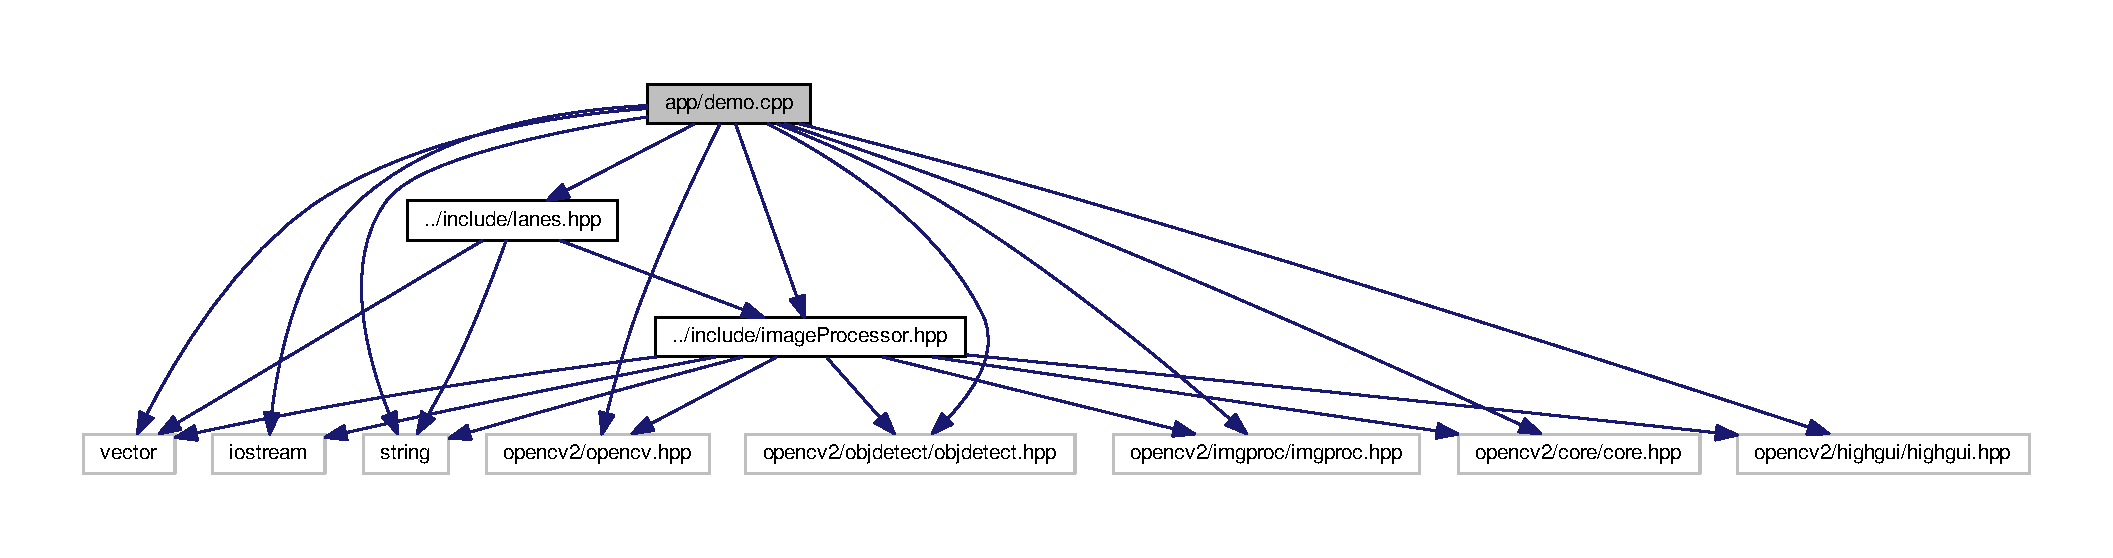
\includegraphics[width=350pt]{demo_8cpp__incl}
\end{center}
\end{figure}
\subsection*{Functions}
\begin{DoxyCompactItemize}
\item 
int \hyperlink{demo_8cpp_a0ddf1224851353fc92bfbff6f499fa97}{main} (int argc, char $\ast$argv\mbox{[}$\,$\mbox{]})
\begin{DoxyCompactList}\small\item\em Function main that runs the main algorithm of the lane detection. \end{DoxyCompactList}\end{DoxyCompactItemize}


\subsection{Detailed Description}
\subsection*{\+: Implements an instance of lane detection application }

============================================================================

\begin{DoxyAuthor}{Author}
\+: Rishabh Choudhary, Akash Atharv 
\end{DoxyAuthor}
\begin{DoxyVersion}{Version}
\+: 1.\+0  \+: M\+IT License  2018 Rishabh Choudhary, Akash Atharv 
\end{DoxyVersion}


\subsection{Function Documentation}
\index{demo.\+cpp@{demo.\+cpp}!main@{main}}
\index{main@{main}!demo.\+cpp@{demo.\+cpp}}
\subsubsection[{\texorpdfstring{main(int argc, char $\ast$argv[])}{main(int argc, char *argv[])}}]{\setlength{\rightskip}{0pt plus 5cm}int main (
\begin{DoxyParamCaption}
\item[{int}]{argc, }
\item[{char $\ast$}]{argv\mbox{[}$\,$\mbox{]}}
\end{DoxyParamCaption}
)}\hypertarget{demo_8cpp_a0ddf1224851353fc92bfbff6f499fa97}{}\label{demo_8cpp_a0ddf1224851353fc92bfbff6f499fa97}


Function main that runs the main algorithm of the lane detection. 

It will read a video of a car in the highway and it will output the same video but with the plotted detected lane 
\begin{DoxyParams}{Parameters}
{\em argv\mbox{[}$\,$\mbox{]}} & is a string to the full path of the demo video \\
\hline
\end{DoxyParams}
\begin{DoxyReturn}{Returns}
0 for successful execution, -\/1 for failed execution 
\end{DoxyReturn}
Superimpose mask with the edge detected image to generate region of interest image

Convert back the grayscale image to R\+GB for inputting into Hough transform

Apply linear regression on the set of points obtained from separated lines to generate one line on left and right side which form the lane
\hypertarget{imageProcessor_8cpp}{}\section{app/image\+Processor.cpp File Reference}
\label{imageProcessor_8cpp}\index{app/image\+Processor.\+cpp@{app/image\+Processor.\+cpp}}


\subsection*{\+: Contains function definitions of the class \hyperlink{classimageProcessor}{image\+Processor} } 


{\ttfamily \#include \char`\"{}../include/image\+Processor.\+hpp\char`\"{}}\\*
Include dependency graph for image\+Processor.\+cpp\+:
\nopagebreak
\begin{figure}[H]
\begin{center}
\leavevmode
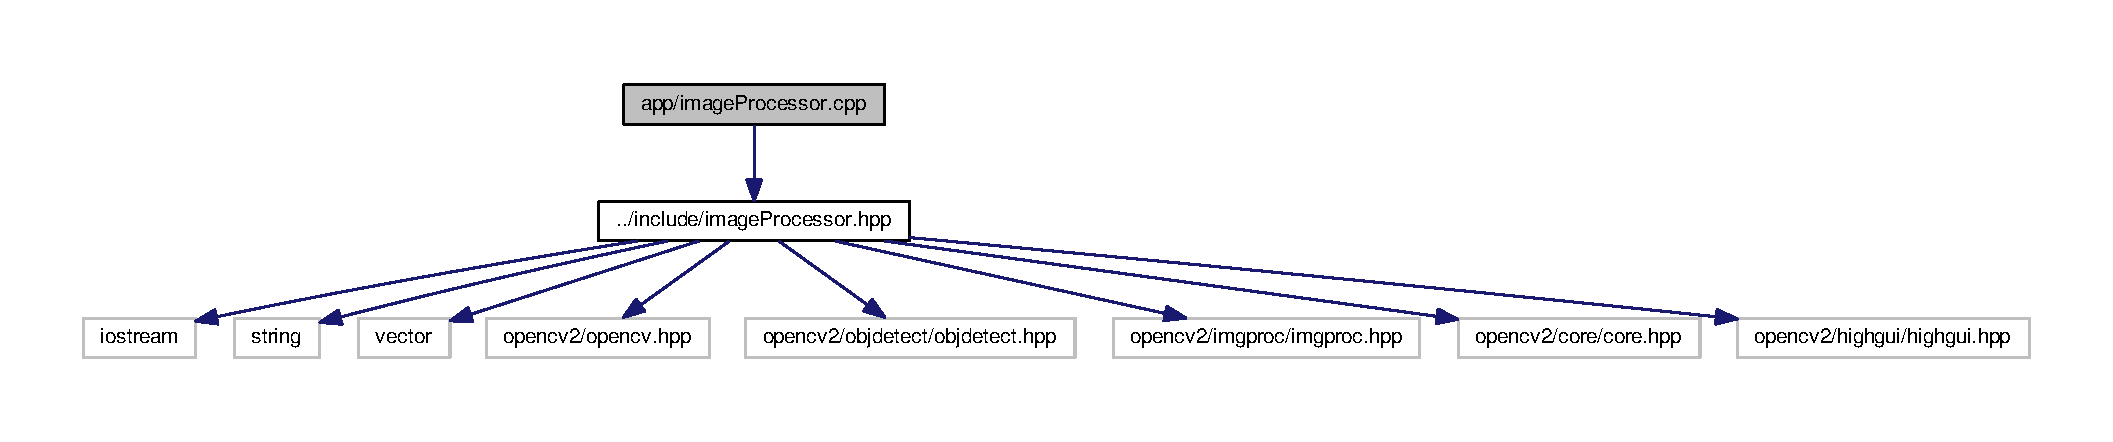
\includegraphics[width=350pt]{imageProcessor_8cpp__incl}
\end{center}
\end{figure}


\subsection{Detailed Description}
\subsection*{\+: Contains function definitions of the class \hyperlink{classimageProcessor}{image\+Processor} }

============================================================================

\begin{DoxyAuthor}{Author}
\+: Rishabh Choudhary, Akash Atharv 
\end{DoxyAuthor}
\begin{DoxyVersion}{Version}
\+: 1.\+0 
\end{DoxyVersion}
\begin{DoxyCopyright}{Copyright}
\+: M\+IT License Copyright 2018 Rishabh Choudhary, Akash Atharv 
\end{DoxyCopyright}

\hypertarget{lanes_8cpp}{}\section{app/lanes.cpp File Reference}
\label{lanes_8cpp}\index{app/lanes.\+cpp@{app/lanes.\+cpp}}


\subsection*{\+: Contains function definitions of the class lanes } 


{\ttfamily \#include $<$lanes.\+hpp$>$}\\*
Include dependency graph for lanes.\+cpp\+:
\nopagebreak
\begin{figure}[H]
\begin{center}
\leavevmode
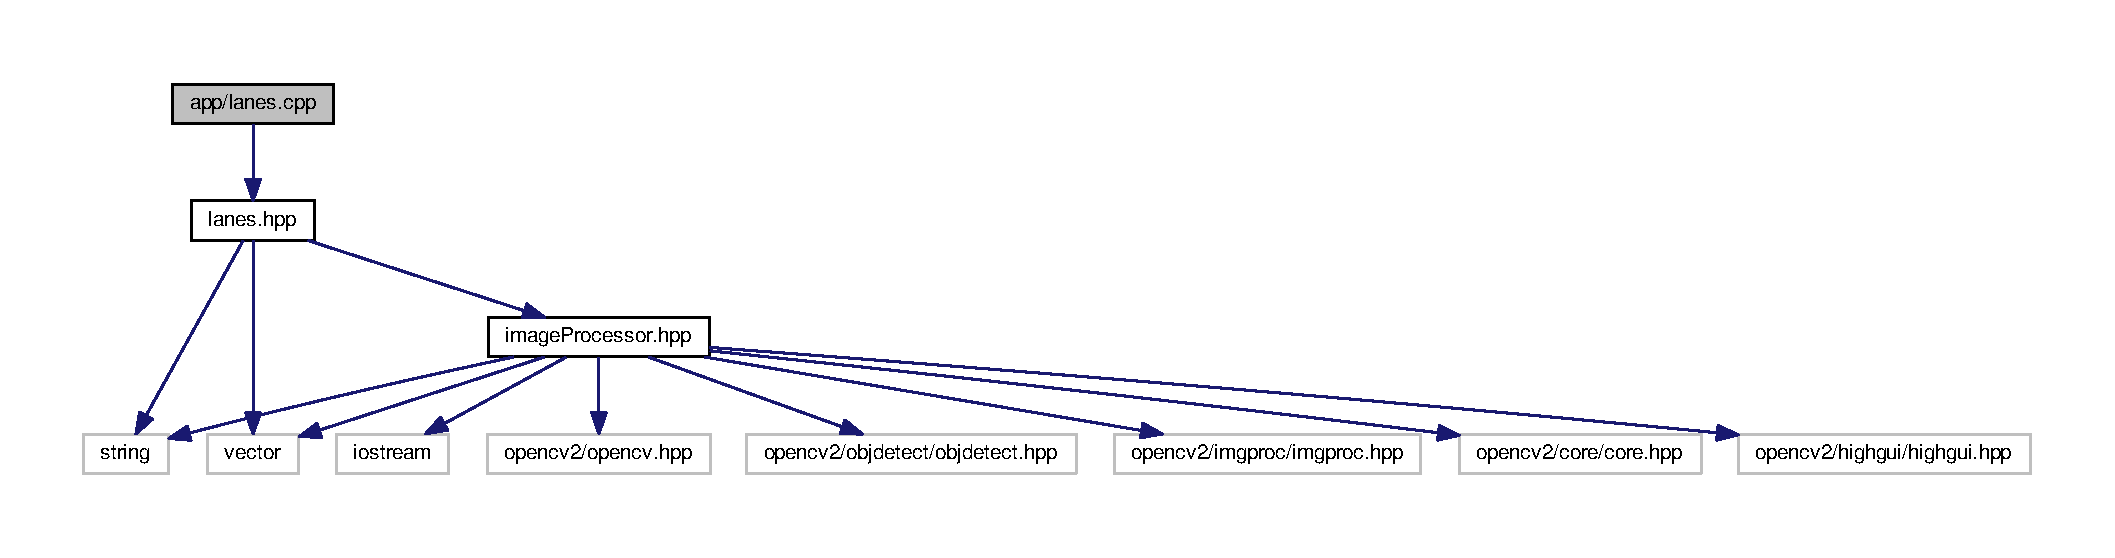
\includegraphics[width=350pt]{lanes_8cpp__incl}
\end{center}
\end{figure}


\subsection{Detailed Description}
\subsection*{\+: Contains function definitions of the class lanes }

============================================================================

\begin{DoxyAuthor}{Author}
\+: Rishabh Choudhary, Akash Atharv 
\end{DoxyAuthor}
\begin{DoxyVersion}{Version}
\+: 1.\+0 
\end{DoxyVersion}
\begin{DoxyCopyright}{Copyright}
\+: M\+IT License Copyright 2018 Rishabh Choudhary, Akash Atharv 
\end{DoxyCopyright}

\hypertarget{imageProcessor_8hpp}{}\section{include/image\+Processor.hpp File Reference}
\label{imageProcessor_8hpp}\index{include/image\+Processor.\+hpp@{include/image\+Processor.\+hpp}}


\subsection*{\+: Contains function and variable declarations of the class \hyperlink{classimageProcessor}{image\+Processor} } 


{\ttfamily \#include $<$iostream$>$}\\*
{\ttfamily \#include $<$string$>$}\\*
{\ttfamily \#include $<$vector$>$}\\*
{\ttfamily \#include \char`\"{}opencv2/opencv.\+hpp\char`\"{}}\\*
{\ttfamily \#include $<$opencv2/objdetect/objdetect.\+hpp$>$}\\*
{\ttfamily \#include $<$opencv2/imgproc/imgproc.\+hpp$>$}\\*
{\ttfamily \#include $<$opencv2/core/core.\+hpp$>$}\\*
{\ttfamily \#include $<$opencv2/highgui/highgui.\+hpp$>$}\\*
Include dependency graph for image\+Processor.\+hpp\+:
\nopagebreak
\begin{figure}[H]
\begin{center}
\leavevmode
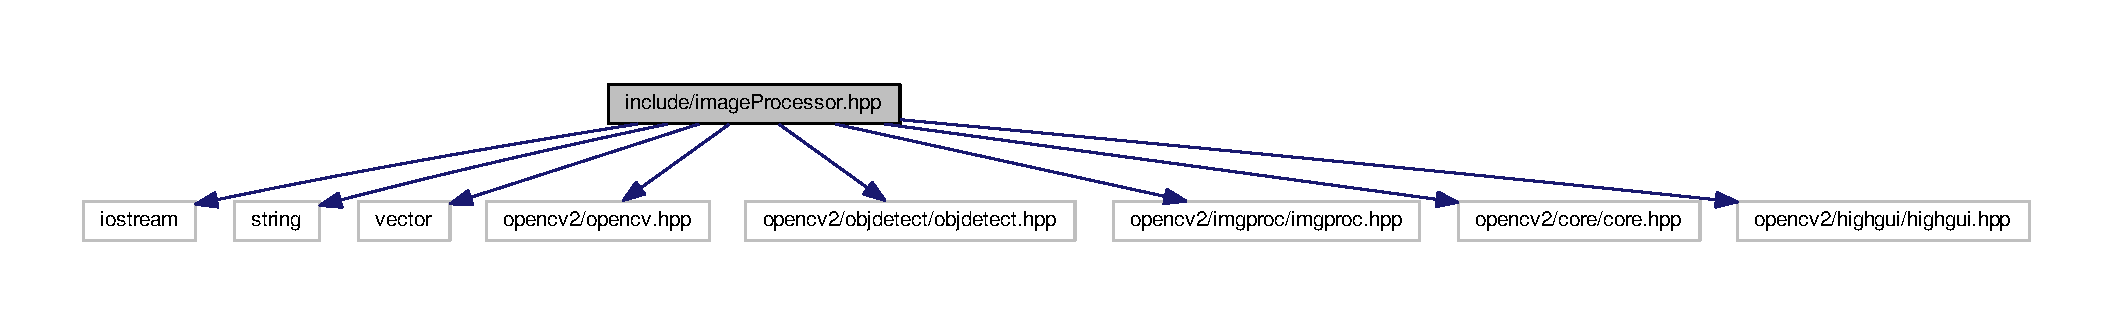
\includegraphics[width=350pt]{imageProcessor_8hpp__incl}
\end{center}
\end{figure}
This graph shows which files directly or indirectly include this file\+:
\nopagebreak
\begin{figure}[H]
\begin{center}
\leavevmode
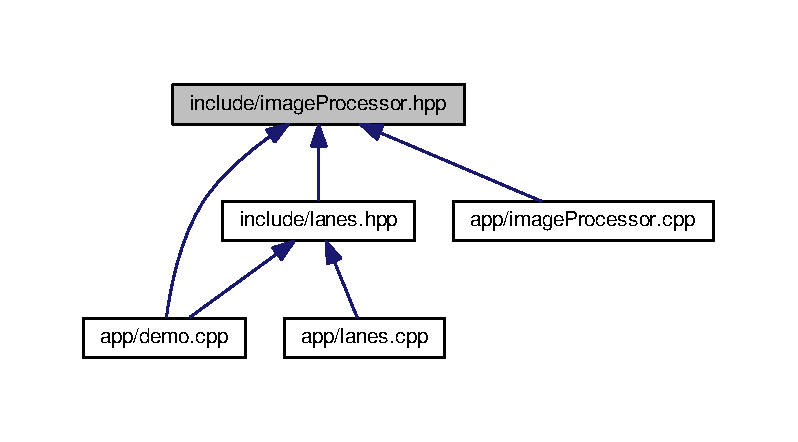
\includegraphics[width=350pt]{imageProcessor_8hpp__dep__incl}
\end{center}
\end{figure}
\subsection*{Classes}
\begin{DoxyCompactItemize}
\item 
class \hyperlink{classimageProcessor}{image\+Processor}
\begin{DoxyCompactList}\small\item\em Class \hyperlink{classimageProcessor}{image\+Processor} The class \hyperlink{classimageProcessor}{image\+Processor} deals with the initial processing algorithms to be performed on the frame before the lines detected are processed further. \end{DoxyCompactList}\end{DoxyCompactItemize}


\subsection{Detailed Description}
\subsection*{\+: Contains function and variable declarations of the class \hyperlink{classimageProcessor}{image\+Processor} }

============================================================================

\begin{DoxyAuthor}{Author}
\+: Rishabh Choudhary, Akash Atharv 
\end{DoxyAuthor}
\begin{DoxyVersion}{Version}
\+: 1.\+0 
\end{DoxyVersion}
\begin{DoxyCopyright}{Copyright}
\+: M\+IT License Copyright 2018 Rishabh Choudhary, Akash Atharv 
\end{DoxyCopyright}

\hypertarget{lanes_8hpp}{}\section{include/lanes.hpp File Reference}
\label{lanes_8hpp}\index{include/lanes.\+hpp@{include/lanes.\+hpp}}


\subsection*{\+: Contains function and variable definitions of the class lanes } 


{\ttfamily \#include $<$string$>$}\\*
{\ttfamily \#include $<$vector$>$}\\*
{\ttfamily \#include $<$image\+Processor.\+hpp$>$}\\*
Include dependency graph for lanes.\+hpp\+:
\nopagebreak
\begin{figure}[H]
\begin{center}
\leavevmode
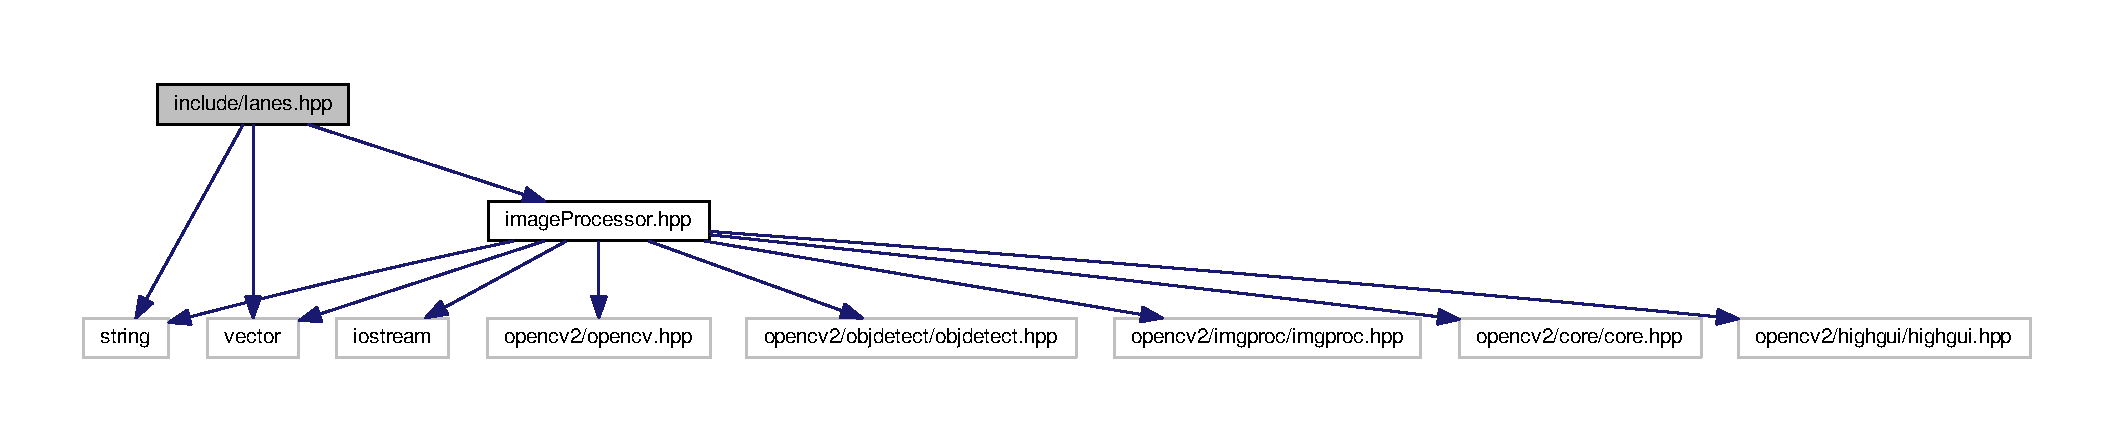
\includegraphics[width=350pt]{lanes_8hpp__incl}
\end{center}
\end{figure}
This graph shows which files directly or indirectly include this file\+:
\nopagebreak
\begin{figure}[H]
\begin{center}
\leavevmode
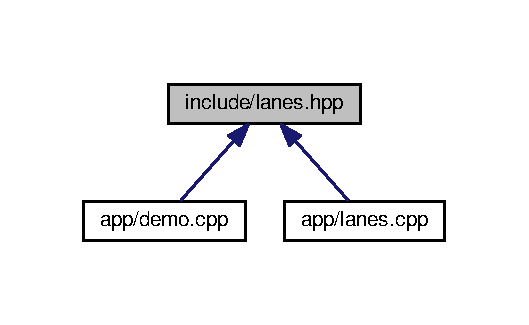
\includegraphics[width=254pt]{lanes_8hpp__dep__incl}
\end{center}
\end{figure}
\subsection*{Classes}
\begin{DoxyCompactItemize}
\item 
class \hyperlink{classlanes}{lanes}
\begin{DoxyCompactList}\small\item\em Class lanes The class lanes deals with all the operations remaining for lane detection after the hough lines in the image have been detected derived from the base class Image\+Processor. \end{DoxyCompactList}\end{DoxyCompactItemize}


\subsection{Detailed Description}
\subsection*{\+: Contains function and variable definitions of the class lanes }

============================================================================

\begin{DoxyAuthor}{Author}
\+: Rishabh Choudhary, Akash Atharv 
\end{DoxyAuthor}
\begin{DoxyVersion}{Version}
\+: 1.\+0 
\end{DoxyVersion}
\begin{DoxyCopyright}{Copyright}
\+: M\+IT License Copyright 2018 Rishabh Choudhary, Akash Atharv 
\end{DoxyCopyright}

%--- End generated contents ---

% Index
\backmatter
\newpage
\phantomsection
\clearemptydoublepage
\addcontentsline{toc}{chapter}{Index}
\printindex

\end{document}
